% F2 — The per-burst lifecycle with GUIDES above and SENSORS below each step (Böckeler's timing
% diagram, drawn vertically: steps top→bottom). Guides steer before the step; sensors check
% after it. Fill: grey = computational (deterministic code: tests, hooks, guards); white =
% inferential (a fresh-context agent); the diamond = the human gate. Dashed = PROPOSED.
% The K-clean-passes → FREEZE decision lives in F4, not here. Census 2026-09-02.
\documentclass[tikz,border=4pt]{standalone}
\usepackage[T1]{fontenc}
\usepackage{lmodern}
\usetikzlibrary{positioning,calc,shapes.geometric,arrows.meta,fit,backgrounds}
\newcommand{\nohyph}{\hyphenpenalty=10000 \exhyphenpenalty=10000 }
\begin{document}
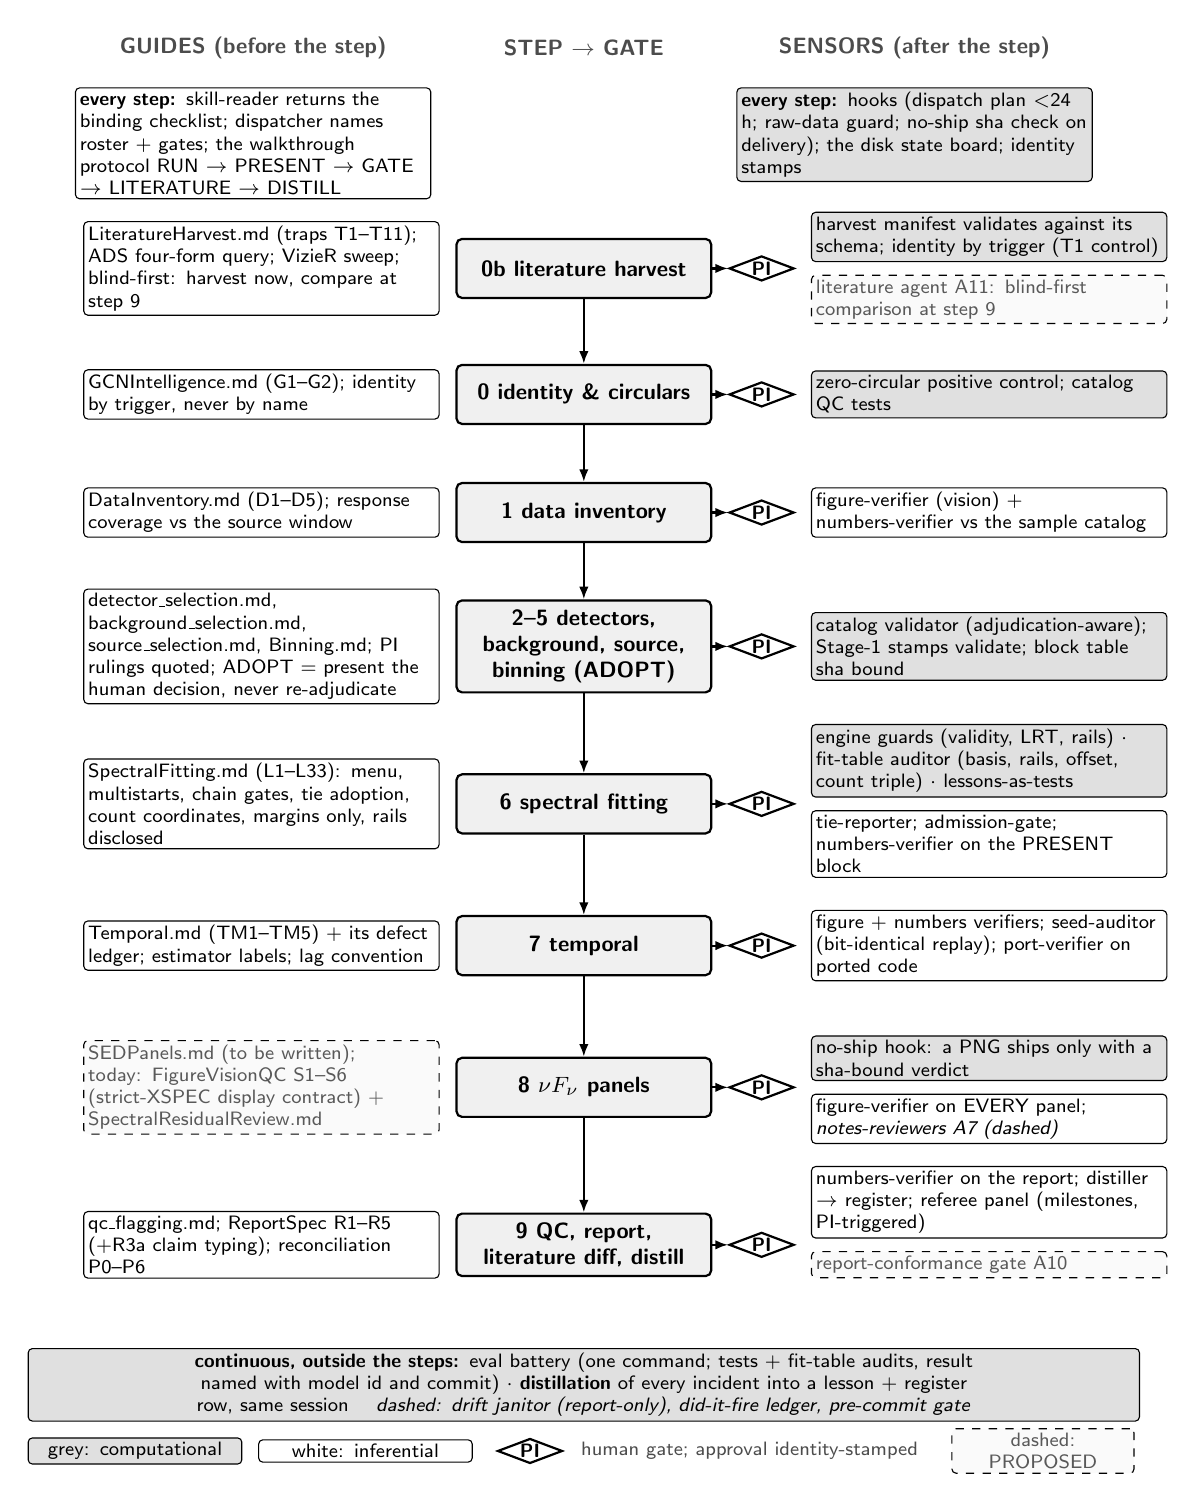
\begin{tikzpicture}[
  font=\sffamily\scriptsize, node distance=1.6mm and 3mm,
  stp/.style={draw, thick, rounded corners=2pt, fill=black!6, text width=30mm, align=center, minimum height=7.5mm, font=\sffamily\footnotesize\bfseries, execute at begin node=\nohyph},
  guide/.style={draw, rounded corners=1.5pt, fill=white, text width=44mm, align=left, inner sep=1.6pt, execute at begin node=\nohyph},
  comp/.style={draw, rounded corners=1.5pt, fill=black!12, text width=44mm, align=left, inner sep=1.6pt, execute at begin node=\nohyph},
  infer/.style={draw, rounded corners=1.5pt, fill=white, text width=44mm, align=left, inner sep=1.6pt, execute at begin node=\nohyph},
  prop/.style={dashed, text=black!65, fill=black!2},
  gate/.style={draw, thick, diamond, aspect=2.6, fill=white, inner sep=0.5pt, font=\sffamily\scriptsize\bfseries},
  arr/.style={-{Latex[length=1.6mm]}, thick},
  lab/.style={font=\sffamily\scriptsize, text=black!70, execute at begin node=\nohyph}]

% column headers
\node[lab, font=\sffamily\footnotesize\bfseries] (hg) at (-42mm,0) {GUIDES (before the step)};
\node[lab, font=\sffamily\footnotesize\bfseries] (hs) at (0,0) {STEP $\to$ GATE};
\node[lab, font=\sffamily\footnotesize\bfseries] (hc) at (42mm,0) {SENSORS (after the step)};

% every step: the cross-cutting guides and sensors, stated once (a band above the rows)
\node[guide, anchor=north] (g0) at (-42mm,-5mm) {\textbf{every step:} skill-reader returns the binding checklist; dispatcher names roster + gates; the walkthrough protocol RUN $\to$ PRESENT $\to$ GATE $\to$ LITERATURE $\to$ DISTILL};
\node[comp, anchor=north] (c0) at (42mm,-5mm) {\textbf{every step:} hooks (dispatch plan $<$24 h; raw-data guard; no-ship sha check on delivery); the disk state board; identity stamps};

% steps at fixed rows
\node[stp] (s0b) at (0,-28mm) {0b literature harvest};
\node[stp] (s0)  at (0,-44mm) {0 identity \& circulars};
\node[stp] (s1)  at (0,-59mm) {1 data inventory};
\node[stp] (s25) at (0,-76mm) {2--5 detectors, background, source, binning (ADOPT)};
\node[stp] (s6)  at (0,-96mm) {6 spectral fitting};
\node[stp] (s7)  at (0,-114mm) {7 temporal};
\node[stp] (s8)  at (0,-132mm) {8 $\nu F_\nu$ panels};
\node[stp] (s9)  at (0,-152mm) {9 QC, report, literature diff, distill};

% gates (one per step, to the right of the step)
\foreach \s in {s0b,s0,s1,s25,s6,s7,s8,s9} {
  \node[gate, right=2mm of \s] (g\s) {PI};
}

% guides per step (left)
\node[guide, left=2mm of s0b] (gl0b) {LiteratureHarvest.md (traps T1--T11); ADS four-form query; VizieR sweep; blind-first: harvest now, compare at step 9};
\node[guide, left=2mm of s0] (gl0) {GCNIntelligence.md (G1--G2); identity by trigger, never by name};
\node[guide, left=2mm of s1] (gl1) {DataInventory.md (D1--D5); response coverage vs the source window};
\node[guide, left=2mm of s25] (gl25) {detector\_selection.md, background\_selection.md, source\_selection.md, Binning.md; PI rulings quoted; ADOPT = present the human decision, never re-adjudicate};
\node[guide, left=2mm of s6] (gl6) {SpectralFitting.md (L1--L33): menu, multistarts, chain gates, tie adoption, count coordinates, margins only, rails disclosed};
\node[guide, left=2mm of s7] (gl7) {Temporal.md (TM1--TM5) + its defect ledger; estimator labels; lag convention};
\node[guide, left=2mm of s8, prop] (gl8) {SEDPanels.md (to be written); today: FigureVisionQC S1--S6 (strict-XSPEC display contract) + SpectralResidualReview.md};
\node[guide, left=2mm of s9] (gl9) {qc\_flagging.md; ReportSpec R1--R5 (+R3a claim typing); reconciliation P0--P6};

% sensors per step (right of the gate); grey = code, white = agent; stacked where a step has both
\node[comp, anchor=south west] (sr0ba) at ($(gs0b.east)+(2mm,0.8mm)$) {harvest manifest validates against its schema; identity by trigger (T1 control)};
\node[infer, prop, anchor=north west] (sr0bb) at ($(gs0b.east)+(2mm,-0.8mm)$) {literature agent A11: blind-first comparison at step 9};
\node[comp, right=2mm of gs0] (sr0) {zero-circular positive control; catalog QC tests};
\node[infer, right=2mm of gs1] (sr1) {figure-verifier (vision) + numbers-verifier vs the sample catalog};
\node[comp, right=2mm of gs25] (sr25) {catalog validator (adjudication-aware); Stage-1 stamps validate; block table sha bound};
\node[comp, anchor=south west] (sr6a) at ($(gs6.east)+(2mm,0.8mm)$) {engine guards (validity, LRT, rails) $\cdot$ fit-table auditor (basis, rails, offset, count triple) $\cdot$ lessons-as-tests};
\node[infer, anchor=north west] (sr6b) at ($(gs6.east)+(2mm,-0.8mm)$) {tie-reporter; admission-gate; numbers-verifier on the PRESENT block};
\node[infer, right=2mm of gs7] (sr7) {figure + numbers verifiers; seed-auditor (bit-identical replay); port-verifier on ported code};
\node[comp, anchor=south west] (sr8a) at ($(gs8.east)+(2mm,0.8mm)$) {no-ship hook: a PNG ships only with a sha-bound verdict};
\node[infer, anchor=north west] (sr8b) at ($(gs8.east)+(2mm,-0.8mm)$) {figure-verifier on EVERY panel; \textit{notes-reviewers A7 (dashed)}};
\node[infer, anchor=south west] (sr9a) at ($(gs9.east)+(2mm,0.8mm)$) {numbers-verifier on the report; distiller $\to$ register; referee panel (milestones, PI-triggered)};
\node[infer, prop, anchor=north west] (sr9b) at ($(gs9.east)+(2mm,-0.8mm)$) {report-conformance gate A10};

% flow arrows: step -> gate -> next step
\foreach \a/\b in {s0b/s0, s0/s1, s1/s25, s25/s6, s6/s7, s7/s8, s8/s9} { \draw[arr] (\a) -- (\b); }
\foreach \s in {s0b,s0,s1,s25,s6,s7,s8,s9} { \draw[arr] (\s.east) -- (g\s.west); }

% continuous band at the bottom
\node[comp, below=9mm of s9, text width=140mm, align=center] (band) {\textbf{continuous, outside the steps:} eval battery (one command; tests + fit-table audits, result named with model id and commit) $\cdot$ \textbf{distillation} of every incident into a lesson + register row, same session \quad\textit{dashed: drift janitor (report-only), did-it-fire ledger, pre-commit gate}};

% legend
\node[comp, below=2mm of band.south west, anchor=north west, text width=26mm, align=center] (l1) {grey: computational};
\node[infer, right=2mm of l1, text width=26mm, align=center] (l2) {white: inferential};
\node[gate, right=3mm of l2] (l3) {PI};
\node[lab, right=1mm of l3] (l3t) {human gate; approval identity-stamped};
\node[infer, prop, right=3mm of l3t, text width=22mm, align=center] (l4) {dashed: PROPOSED};
\end{tikzpicture}
\end{document}
